% !TeX program = pdfLaTeX
\documentclass[smallextended]{svmult}       % onecolumn (second format)
%\documentclass[twocolumn]{svjour3}          % twocolumn
%
\smartqed  % flush right qed marks, e.g. at end of proof
%
\usepackage{amsmath}
\usepackage{graphicx}
\usepackage[utf8]{inputenc}

\usepackage[hyphens]{url} % not crucial - just used below for the URL
\usepackage{hyperref}
\providecommand{\tightlist}{%
  \setlength{\itemsep}{0pt}\setlength{\parskip}{0pt}}

%
% \usepackage{mathptmx}      % use Times fonts if available on your TeX system
%
% insert here the call for the packages your document requires
%\usepackage{latexsym}
% etc.
%
% please place your own definitions here and don't use \def but
% \newcommand{}{}
%
% Insert the name of "your journal" with
% \journalname{myjournal}
%

%% load any required packages here


\usepackage{color}
\usepackage{fancyvrb}
\newcommand{\VerbBar}{|}
\newcommand{\VERB}{\Verb[commandchars=\\\{\}]}
\DefineVerbatimEnvironment{Highlighting}{Verbatim}{commandchars=\\\{\}}
% Add ',fontsize=\small' for more characters per line
\usepackage{framed}
\definecolor{shadecolor}{RGB}{248,248,248}
\newenvironment{Shaded}{\begin{snugshade}}{\end{snugshade}}
\newcommand{\KeywordTok}[1]{\textcolor[rgb]{0.13,0.29,0.53}{\textbf{#1}}}
\newcommand{\DataTypeTok}[1]{\textcolor[rgb]{0.13,0.29,0.53}{#1}}
\newcommand{\DecValTok}[1]{\textcolor[rgb]{0.00,0.00,0.81}{#1}}
\newcommand{\BaseNTok}[1]{\textcolor[rgb]{0.00,0.00,0.81}{#1}}
\newcommand{\FloatTok}[1]{\textcolor[rgb]{0.00,0.00,0.81}{#1}}
\newcommand{\ConstantTok}[1]{\textcolor[rgb]{0.00,0.00,0.00}{#1}}
\newcommand{\CharTok}[1]{\textcolor[rgb]{0.31,0.60,0.02}{#1}}
\newcommand{\SpecialCharTok}[1]{\textcolor[rgb]{0.00,0.00,0.00}{#1}}
\newcommand{\StringTok}[1]{\textcolor[rgb]{0.31,0.60,0.02}{#1}}
\newcommand{\VerbatimStringTok}[1]{\textcolor[rgb]{0.31,0.60,0.02}{#1}}
\newcommand{\SpecialStringTok}[1]{\textcolor[rgb]{0.31,0.60,0.02}{#1}}
\newcommand{\ImportTok}[1]{#1}
\newcommand{\CommentTok}[1]{\textcolor[rgb]{0.56,0.35,0.01}{\textit{#1}}}
\newcommand{\DocumentationTok}[1]{\textcolor[rgb]{0.56,0.35,0.01}{\textbf{\textit{#1}}}}
\newcommand{\AnnotationTok}[1]{\textcolor[rgb]{0.56,0.35,0.01}{\textbf{\textit{#1}}}}
\newcommand{\CommentVarTok}[1]{\textcolor[rgb]{0.56,0.35,0.01}{\textbf{\textit{#1}}}}
\newcommand{\OtherTok}[1]{\textcolor[rgb]{0.56,0.35,0.01}{#1}}
\newcommand{\FunctionTok}[1]{\textcolor[rgb]{0.00,0.00,0.00}{#1}}
\newcommand{\VariableTok}[1]{\textcolor[rgb]{0.00,0.00,0.00}{#1}}
\newcommand{\ControlFlowTok}[1]{\textcolor[rgb]{0.13,0.29,0.53}{\textbf{#1}}}
\newcommand{\OperatorTok}[1]{\textcolor[rgb]{0.81,0.36,0.00}{\textbf{#1}}}
\newcommand{\BuiltInTok}[1]{#1}
\newcommand{\ExtensionTok}[1]{#1}
\newcommand{\PreprocessorTok}[1]{\textcolor[rgb]{0.56,0.35,0.01}{\textit{#1}}}
\newcommand{\AttributeTok}[1]{\textcolor[rgb]{0.77,0.63,0.00}{#1}}
\newcommand{\RegionMarkerTok}[1]{#1}
\newcommand{\InformationTok}[1]{\textcolor[rgb]{0.56,0.35,0.01}{\textbf{\textit{#1}}}}
\newcommand{\WarningTok}[1]{\textcolor[rgb]{0.56,0.35,0.01}{\textbf{\textit{#1}}}}
\newcommand{\AlertTok}[1]{\textcolor[rgb]{0.94,0.16,0.16}{#1}}
\newcommand{\ErrorTok}[1]{\textcolor[rgb]{0.64,0.00,0.00}{\textbf{#1}}}
\newcommand{\NormalTok}[1]{#1}

\usepackage{float} \usepackage{url} \floatplacement{figure}{H}

\begin{document}

\title{Exploring population structure with admixture models and principal
components analysis }


    \titlerunning{Exploring population structure with ADMIXTURE and PCA}

%\author{  Chi-Chun Liu \and  Suyash Shringapure \and  Kenneth Lange \and  John Novembre }


%\institute{
%        Chi-Chun Liu \at Department of Human Genetics, University of Chicago, Chicago, IL.
%    \and
%        Suyash Shringapure \at 23andme, Mountain View, CA.
%    \and
%        Kenneth Lange \at Departments of Biomathematics, Human Genetics, and Statistics.
% University of California, Los Angeles, Los Angeles, CA.
%    \and
%        John Novembre \at Department of Human Genetics, Ecology and Evolution. University of  Chicago. Chicago, IL.
%    }


\maketitle

\begin{abstract}
Population structure is a commonplace feature of genetic variation data,
and it has importance in numerous application areas, including
evolutionary genetics, conservation genetics, and human genetics.
Understanding the structure in a sample is necessary before more
sophisticated analyses are undertaken. Here we provide a protocol for
running principal component analysis (PCA) and admixture proportion
inference - two of the most commonly used approaches in describing
population structure. Along with hands-on examples with CEPH-Human
Genome Diversity Panel and pragmatic caveats, readers will be able to
analyze, and visualize population structure on their own data.
\end{abstract}

%\keywords{
%        population structure \and
%        admixture \and
%        principal component analysis \and
%        population stratification \and
%    }



\def\spacingset#1{\renewcommand{\baselinestretch}%
{#1}\small\normalsize} \spacingset{1}


\section{Introduction}\label{introduction}

Population structure is a commonplace feature of genetic variation data,
and it has importance in numerous application areas, including
evolutionary genetics, conservation genetics, and human genetics. At a
broad level, population structure is the existence of differing levels
of genetic relatedness among some subgroups within a sample. This may
arise for a variety of reasons, but a common cause is that samples have
been drawn from geographically isolated groups or different locales
across a geographic continuum. Regardless of the cause, understanding
the structure in a sample is necessary before more sophisticated
analyses are undertaken. For example, to infer divergence times between
two populations requires knowing two populations even exist and which
individuals belong to each.

Two of the most commonly used approaches to describe population
structure in a sample are principal components analysis \cite{Menozzi78,CavSforza94,Price06,Patterson06} and admixture
proportion inference \cite{Pritchard00,Novembre16}.
In brief, principal components analysis reduces a
multi-dimensional dataset to a much smaller number of dimensions that
allows for visual exploration and compact quantitative summaries. In its
application to genetic data, the numerous genotypes observed per
individual are reduced to a few summary coordinates. With admixture
proportion inference, individuals in a sample are modeled as having a
proportion of their genome derived from each of several source
populations. The goal is to infer the proportions of ancestry in each
source populations, and these proportions can be used to produce compact
visual summaries that reveal the existence of population structure in a
sample.

The history and basic behaviors of both these approaches have been
written about extensively, including by some of us, and so we refer
readers to several previous publications to learn the basic background
and interpretative nuances of these approaches and their derivatives
\cite{Pritch00,Falush03,Rosenberg05,Hubisz09,Raj14,Novembre14,Falush16,Alexander09,Alexander11,Price06,Patterson06,Novembre08,McVean09,Novembre16}.
Here, in the
spirit of this volume, we provide a protocol for running these analyses
and share some pragmatic caveats that do not always arise in more
abstract discussions regarding these methods.

\section{Materials}\label{materials}

The protocol we present is based on two pieces of software: 1) the
\texttt{ADMIXTURE} software that our team developed \cite{Alexander09}
for efficiently estimating admixture
proportions in the ``Pritchard-Stephens-Donnelly'' model of admixture
\cite{Pritchard00,Novembre16}. 2) The
\texttt{smartpca} software developed by Nick Patterson and colleagues
for carrying out PCA \cite{Price06}. Both of these pieces of
software are used widely. We also pair them with downstream tools for
visualization, in particular \texttt{pong} \cite{Behr16}, for
visualizing output of admixture proportion inferences, and
\texttt{PCAviz} \cite{Williams17}, a novel R package for plotting
PCA outputs. We also use \texttt{PLINK} \cite{Purcell07,Chang15} as a tool to perform some basic manipulations of the data
(See Chapter 3 for more background on \texttt{PLINK}).

The example data we use is derived from publicly available
single-nucleotide polymorphism (SNP) genotype data from the CEPH-Human
Genome Diversity Panel \cite{Cann02}. Specifically, we will look at
Illumina 650Y genotyping array data as first described by Li et al \cite{Li08}.
This sample is a global-scale sampling of human diversity
with 52 populations in total, and the raw files are available from the
following link: \url{http://hagsc.org/hgdp/files.html}. These data have
been used in numerous subsequent publications and are an important
reference set.

A few technical details are that the genotypes were filtered with a
cutoff of 0.25 for the Illumina GenCall score \cite{GenCall} (a quality
score generated by the basic genotype calling software). Further,
individuals with a genotype call rate \textless{}98.5\% were removed,
with the logic being that if a sample has many missing genotypes it may
due to poor quality of the source DNA, and so none of the genotypes from
that individual should be trusted. Beyond this, to prepare the data, we
have filtered down the individuals to a set of 938 unrelated
individuals. We exclude related individuals as we are not interested in
population structure that is due to family relationships and methods
such as PCA and \texttt{ADMIXTURE} can inadvertently mistake family
structure for population structure. The starting data are available as
plink-formatted files \texttt{H938.bed} \texttt{H938.fam},
\texttt{H938.bim}, and an accompanying set of population identifiers
\texttt{H938.clst.txt} in the \texttt{raw\_input} sub-directory of the
repository.

As a pragmatic side note, it is common (and recommended) when carrying
out analyses of population structure to merge one's data with other
datasets that contain populations which may be representative sources of
admixing individuals. For example, in analyzing a dataset with African
American individuals, it can be helpful to include datasets containing
African and European individuals in the analysis. These datasets can be
merged with your dataset using software such as \texttt{plink}. However,
when merging several datasets, one should be aware of potential biases
that can be introduced due to strand flips (i.e.~one dataset reports
genotypes on the `+' strand of the reference human genome, and another
on the `-' strand). One precautionary step to detect strand flips is to
group individuals by what dataset they derive from and then produce a
scatterplot of allele frequencies for pairs of groups at a time. If
strand flips are not being controlled correctly, one will observe
numerous variants on the \(y=1-x\) line, where \(x\) is the frequency in
one dataset and \(y\) is the frequency in a second dataset. (Note: this
rule of thumb assumes levels of differentiation are low between
datasets, as is the case in human datasets in general, but one should
still keep this in mind interpreting results).

\section{Methods}\label{methods}

In this section we walk you through an example analysis using
\texttt{ADMIXTURE} and \texttt{smartpca}. We assume the raw data files
are in a directory \texttt{raw\_input} that is below our working
directory and that second directory \texttt{out} exists in which outputs
can be placed. If following along in an \texttt{R} console, you should
use the \texttt{setwd()} command to set the working directory correctly.

\subsection{Subsetting Data}\label{subsetting-data}

For running some simple examples below, we will first create a subset of
the HGDP sample that is restricted to only European populations. The
European populations in the HGDP have the labels `Adygei', `Basque',
`French', `Italian', `Orcadian', `Russian', `Sardinian' and `Tuscan', so
we create a list of individuals matching these labels using an
\texttt{awk} command, and then use \texttt{plink}`s \texttt{-\/-keep}
option to make a new dataset with output prefix 'H938\_Euro'.

\begin{Shaded}
\begin{Highlighting}[]
\FunctionTok{awk} \StringTok{'$3=="Adygei"||$3=="French_Basque"||$3=="French"|| \textbackslash{}}
\StringTok{$3=="North_Italian"||$3=="Orcadian"||$3=="Russian"|| \textbackslash{} }
\StringTok{$3=="Sardinian"||$3=="Tuscan" \{print $0\}'}\NormalTok{ \textbackslash{}}
\NormalTok{raw_input/H938.clst.txt }\OperatorTok{>}\NormalTok{ out/Euro.clst.txt}

\ExtensionTok{plink}\NormalTok{ --bfile raw_input/H938 --keep out/Euro.clst.txt }\DataTypeTok{\textbackslash{} }
\ExtensionTok{--make-bed}\NormalTok{ --out out/H938_Euro}
\end{Highlighting}
\end{Shaded}

\subsection{Filter out SNPs to remove linkage disequilibrium
(LD)}\label{filter-out-snps-to-remove-linkage-disequilibrium-ld}

SNPs in high LD with each other contain redundant information. More
worrisome is the potential for some regions of the genome to have a
disproportionate influence on the results and thus distort the
representation of genome-wide structure. A nice empirical example of the
problem is in Figure 5 of Tian et al (Tian et al. 2008), where PC2 of
the genome-wide data is shown to be reflecting the variation in a 3.8Mb
region of chromosome 8 that is known to harbor an inversion. A standard
approach to address this issue is to filter out SNPs based on pairwise
LD to produce a reduced set of more independent markers. Here we use
\texttt{plink}'s commands to produce a new LD-pruned dataset with output
prefix \texttt{H938\_Euro.LDpruned}. The approach considers a
chromosomal window of 50 SNPs at a time, and for any pair whose
genotypes have an association \(r^2\) value greater than 0.1, it removes
a SNP from the pair. Then the window is shifted by 10 SNPs and the
procedure is repeated:

\begin{Shaded}
\begin{Highlighting}[]
\ExtensionTok{plink}\NormalTok{ --bfile out/H938_Euro --indep-pairwise 50 10 0.1}
\ExtensionTok{plink}\NormalTok{ --bfile out/H938_Euro --extract plink.prune.in --make-bed \textbackslash{}}
\NormalTok{--out out/H938_Euro.LDprune}
\end{Highlighting}
\end{Shaded}

(Advanced note: For particularly sensitive results, we recommend
additional rounds of SNP filtering based on observed principal component
loadings and/or population differentiation statistics. For example, a
robust approach is to filter out large windows around any SNP with a
high PCA loading, see Novembre et al. 2008).

\subsection{\texorpdfstring{Running
\texttt{ADMIXTURE}}{Running ADMIXTURE}}\label{running-admixture}

\subsubsection{An example run with
visualization}\label{an-example-run-with-visualization}

The \texttt{ADMIXTURE} software (v 1.3.0 here) comes as a pre-compiled
binary executable file for either Linux or Mac operating systems. To
install, simply download the package and move the executable into your
standard execution path (e.g. `/usr/local/bin' on many linux systems).
Once installed, it is straightforward to run \texttt{ADMIXTURE} with a
fixed number of source populations, commonly denoted by \(K\). For
example, to get started let's run ADMIXTURE with \(K\)=6:

\begin{Shaded}
\begin{Highlighting}[]
\ExtensionTok{admixture}\NormalTok{ out/H938_Euro.LDprune.bed 6}
\end{Highlighting}
\end{Shaded}

\texttt{ADMIXTURE} is a maximum-likelihood based method, so as the
method runs, you will see updates to the log-likelihood as it converges
on a solution for the ancestry proportions and allele frequencies that
maximize the likelhood function. The algorithm will stop when the
difference between successive iterations is small (the `delta' value
takes a small value). A final output is an estimated \(F_{ST}\) value
(Holsinger and Weir 2009) between each of the source populations, based
on the inferred allele frequencies. These estimates reflect how
differentiated the source populations are, which is important for
understanding whether the population structure observed in a sample is
substantial or not (values closer to 0 reflect less population
differentiation).

After running, \texttt{ADMIXTURE} produces two major output files. The
file with suffix \texttt{.P} contains an \(L \times K\) table of the
allele frequencies inferred for each SNP in each population. The file
with suffix \texttt{.Q} contains an \(N \times K\) table of inferred
individual ancestry proportions from the \(K\) ancestral populations,
with one row per individual.

For our example dataset with \(K\)=6, this will be a file called
\texttt{H938.LDpruned.6.Q}. This file can be used to generate a plot
showing individual ancestry. In \texttt{R}, this can be done using the
following commands:

\begin{Shaded}
\begin{Highlighting}[]
\KeywordTok{library}\NormalTok{(RColorBrewer)}
\NormalTok{tbl <-}\StringTok{ }\KeywordTok{read.table}\NormalTok{(}\StringTok{"out/H938_Euro.LDprune.6.Q"}\NormalTok{)}
\KeywordTok{par}\NormalTok{(}\DataTypeTok{mar =} \KeywordTok{c}\NormalTok{(}\FloatTok{1.5}\NormalTok{, }\DecValTok{4}\NormalTok{, }\FloatTok{2.5}\NormalTok{, }\DecValTok{2}\NormalTok{),}\DataTypeTok{cex.lab=}\FloatTok{0.75}\NormalTok{,}\DataTypeTok{cex.axis=}\FloatTok{0.6}\NormalTok{)}
\KeywordTok{barplot}\NormalTok{(}\KeywordTok{t}\NormalTok{(}\KeywordTok{as.matrix}\NormalTok{(tbl)),}
  \DataTypeTok{col =} \KeywordTok{brewer.pal}\NormalTok{(}\DecValTok{6}\NormalTok{, }\StringTok{"Set1"}\NormalTok{), }\DataTypeTok{ylab =} \StringTok{"Anc. Proportions"}\NormalTok{,}
  \DataTypeTok{border =} \OtherTok{NA}\NormalTok{, }\DataTypeTok{space =} \DecValTok{0}
\NormalTok{)}
\end{Highlighting}
\end{Shaded}

\begin{figure}
\centering
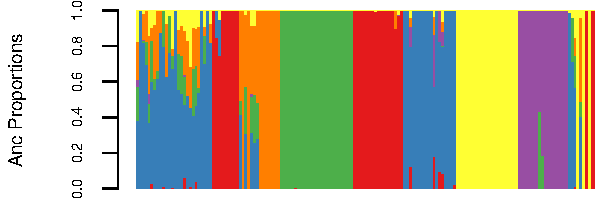
\includegraphics{plot/unnamed-chunk-4-1.pdf}
\caption{Initial rough plot of the ADMIXTURE results for K=6 using R
base graphics.}
\end{figure}

Each thin vertical line in the barplot represents one individual and
each color represents one inferred ancestral population. The length of
each color in a vertical bar represents the proportion of that
individual's ancestry that is derived from the inferred ancestral
population corresponding to that color. The above image suggests there
are some genetic clusters in the data, but it's not a well-organized
data display.

To improve the visualization, one can use a package dedicated to
plotting ancestry proportions (Noah A. Rosenberg 2004; Kopelman et al.
2015; Behr et al. 2016). Here we use a post-processing tool
\texttt{pong} (Behr et al. 2016), which visualizes individual ancestry
with similarity between individuals within clusters. You will most
likely want to install \texttt{pong} on a local machine as it
initializes a local web server to display the results.

To run \texttt{pong} requires setting up a few files: 1) an
\texttt{ind2pop} file that maps individuals to populations; 2) a
\texttt{Qfilemap} file that points \texttt{pong} towards which `.Q'
files to display; These are easy to build up from the command-line using
the \texttt{Euro.clst.txt} file we built above, and an \texttt{awk}
command to output tab-separated text to a file with the
\texttt{Qfilemap} suffix added to whatever file prefix we're using to
organize our runs:

\begin{Shaded}
\begin{Highlighting}[]
\FunctionTok{cut}\NormalTok{ -d}\StringTok{' '}\NormalTok{ -f3 out/Euro.clst.txt }\OperatorTok{>}\NormalTok{ out/H938_Euro.ind2pop}
\VariableTok{FILEPREFIX=}\NormalTok{H938_Euro.LDPrune}
\VariableTok{K=}\NormalTok{6}
\FunctionTok{awk}\NormalTok{ -v K=}\VariableTok{$K}\NormalTok{ -v file=}\VariableTok{$FILEPREFIX} \StringTok{'BEGIN\{ \textbackslash{}}
\StringTok{printf("ExampleRun\textbackslash{}t%d\textbackslash{}t%s.%d.Q\textbackslash{}n",K,file,K) }
\StringTok{\}'} \OperatorTok{>}\NormalTok{ out/}\VariableTok{$FILEPREFIX}\NormalTok{.Qfilemap }
\end{Highlighting}
\end{Shaded}

Note when building the \texttt{.Qfilemap} one needs to use tabs to
separate the columns for \texttt{pong} to read the file correctly.

Then to run \texttt{pong}, we use following command:

\begin{Shaded}
\begin{Highlighting}[]
\ExtensionTok{pong}\NormalTok{ -m out/H938_Euro.LDprune.Qfilemap -i out/H938_Euro.ind2pop}
\end{Highlighting}
\end{Shaded}

We open a web browser to \texttt{http://localhost:4000/} to view the
results.

Here's an example of what you should see:

\begin{figure}
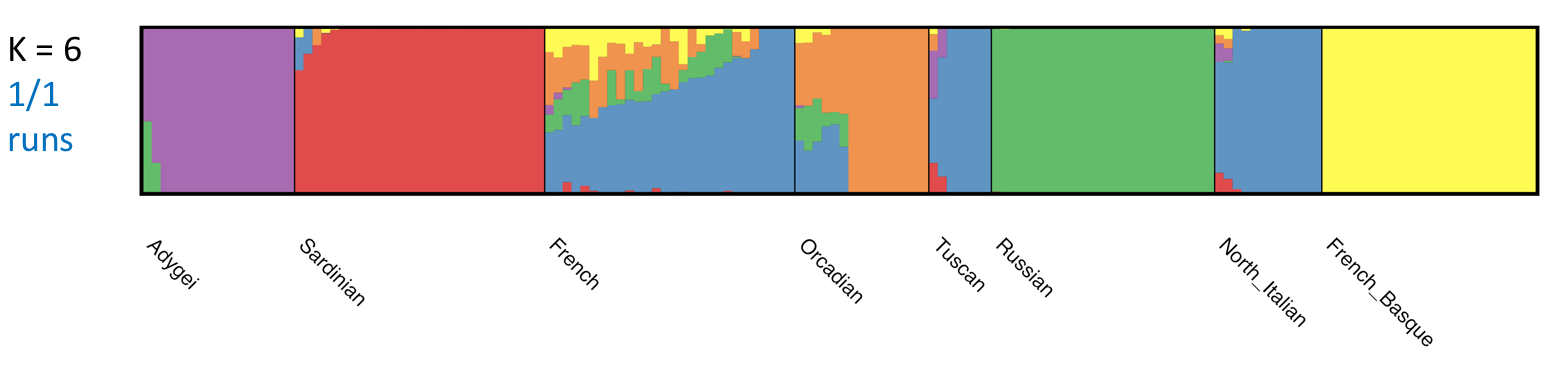
\includegraphics[width=1\linewidth]{./plot/H938_Euro_LDprune_K6} \caption{Plot of the ADMIXTURE results for K=6 using PONG.}\label{fig:unnamed-chunk-7}
\end{figure}

From this visualization, we can see the admixture model fits most
individuals of the Adygei, Sardinian, Russian, French Basque samples as
being derived each from a single source population (represented by
purple, red, green, and yellow respectively). The French, Tuscan, and
North Italian samples are generally estimated to have a majority
component of ancestry from a single source population (blue) though with
admixture with other sources. A first conclusions is that the population
labels do not capture the complexity of the population structure. There
is apparent cryptic structure within some samples (e.g., Orcadian) and
minimal differentiation between other samples (North Italian and Tuscan
samples for instance).

Because ADMIXTURE is a ``greedy'', ``hill-climbing''" optimization
algorithm it is good practice to do multiple runs from different initial
random starting points. We can do this by using the -s flag to specify
the random seed for each ADMIXTURE run.

\begin{Shaded}
\begin{Highlighting}[]
\VariableTok{K=}\NormalTok{6}
\VariableTok{prefix=}\NormalTok{H938_Euro.LDprune}
\CommentTok{# run admixture multiple times}
\KeywordTok{for} \ExtensionTok{r}\NormalTok{ in }\DataTypeTok{\{1..10\}}
\KeywordTok{do}
\ExtensionTok{admixture}\NormalTok{ -s }\VariableTok{$\{RANDOM\}}\NormalTok{ out/H938_Euro.LDprune.bed }\VariableTok{$K}
\FunctionTok{mv}\NormalTok{ out/}\VariableTok{$\{prefix\}}\NormalTok{.}\VariableTok{$\{K\}}\NormalTok{.Q out/}\VariableTok{$\{prefix\}}\NormalTok{.K}\VariableTok{$\{K\}}\NormalTok{r}\VariableTok{$\{r\}}\NormalTok{.Q}
\KeywordTok{done}
\end{Highlighting}
\end{Shaded}

Pong has nice functionality for summarizing the output of the multiple
ADMIXTURE runs. It can collect similar solutions into ``modes'' and
display them in ranked order of the number of runs supporting each. In
the interactive version, you use the
\texttt{check\ to\ highlight\ multimodality} checkbox and whiten
populations with ancestry matrices agreeing with the major mode. One can
also click on and visualize only one cluster. Here we set up the PONG
input files and show an example output.

\begin{Shaded}
\begin{Highlighting}[]
\VariableTok{K=}\NormalTok{6}
\VariableTok{prefix=}\NormalTok{H938_Euro.LDprune}
\CommentTok{# create a pong parameter file}
\KeywordTok{for} \ExtensionTok{r}\NormalTok{ in }\DataTypeTok{\{1..10\}}
\KeywordTok{do}
\FunctionTok{awk}\NormalTok{ -v K=}\VariableTok{$K}\NormalTok{ -v r=}\VariableTok{$r}\NormalTok{ -v file=}\VariableTok{$\{prefix\}}\NormalTok{.K}\VariableTok{$\{K\}}\NormalTok{r}\VariableTok{$\{r\}} \StringTok{'BEGIN\{ \textbackslash{}}
\StringTok{printf("K%dr%d\textbackslash{}t%d\textbackslash{}t%s.Q\textbackslash{}n",K,r,K,file)}
\StringTok{\}'} \OperatorTok{>>}\NormalTok{ out/}\VariableTok{$\{prefix\}}\NormalTok{.k6multiplerun.Qfilemap}
\KeywordTok{done}
\CommentTok{# run pong}
\ExtensionTok{pong}\NormalTok{ -m out/}\VariableTok{$\{prefix\}}\NormalTok{.k6multiplerun.Qfilemap --greedy -s .95 \textbackslash{}}
\NormalTok{-i out/H938_Euro.ind2pop}
\end{Highlighting}
\end{Shaded}

\begin{figure}
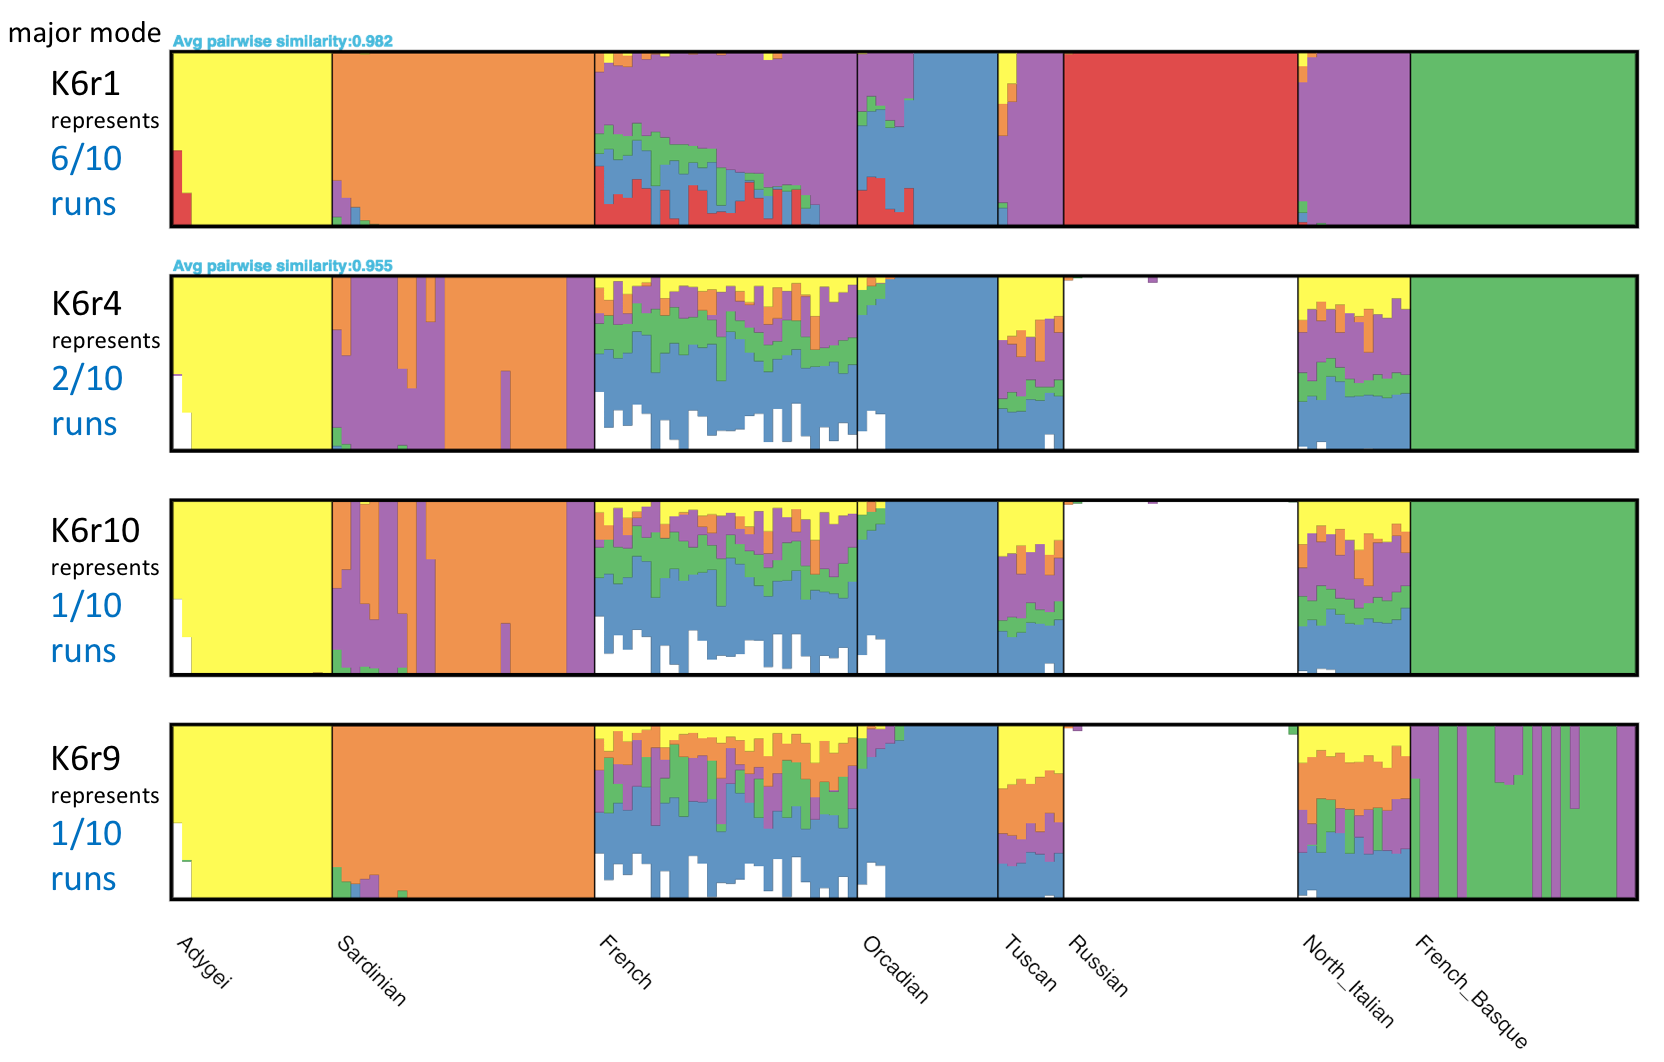
\includegraphics[width=1\linewidth]{./plot/H938_Euro_LDprune_K6_10runs} \caption{PONG plot summarizing multiple ADMIXTURE runs with different random starting points.  The top row shows the major mode (supported by 6 out of 10 runs as indicated in the blue text).  The next three rows show three other solutions found by ADMIXTURE in 2, 1, and 1 runs respectively.}\label{fig:unnamed-chunk-10}
\end{figure}

The resulting figure shows that 6 out of 10 runs converged to the same
mode, which appears equivalent to our initial run above. We observe the
appearance of structure within Sardinia in the second and third modes.
The original run had North Italian and Tuscan samples as a mostly
unadmixed, while all 3 minor modes model the two population as highly
admixed. The fourth mode (supporting by just one run) inferred
sub-structure within the French Basque sample. This instability in the
solution is a hint that the ADMIXTURE model with K=6 is not a perfect
fit to this data.

\subsubsection{\texorpdfstring{Considering different values of
\(K\)}{Considering different values of K}}\label{considering-different-values-of-k}

In a typical analysis, one wants to explore the sensitivity of the
results to the choice of \(K\). One approach is to run ADMIXTURE with
various plausible values of \(K\) and compare the performance of results
visually and using cross-validation error rates. Here is a piece of
\texttt{bash} command-line code that will run \texttt{ADMIXTURE} for
values of \(K\) from 2 to 12, and that will build a file with a table of
cross-validation error rates per value of \(K\).

\begin{Shaded}
\begin{Highlighting}[]
\CommentTok{# Run for different values of K}
\VariableTok{prefix=}\NormalTok{H938_Euro.LDprune}
\VariableTok{Klow=}\NormalTok{1}
\VariableTok{Khigh=}\NormalTok{12}
\KeywordTok{for} \KeywordTok{((}\NormalTok{K=}\VariableTok{$Klow}\NormalTok{;K<=}\VariableTok{$Khigh}\NormalTok{;K++}\KeywordTok{))}\NormalTok{; }\KeywordTok{\textbackslash{}}
\KeywordTok{do} 
  \ExtensionTok{admixture}\NormalTok{ --cv out/}\VariableTok{$prefix}\NormalTok{.bed }\VariableTok{$K} \KeywordTok{|} \FunctionTok{tee}\NormalTok{ log.}\VariableTok{$prefix}\NormalTok{.}\VariableTok{$\{K\}}\NormalTok{.out}\KeywordTok{;} 
\KeywordTok{done}
\end{Highlighting}
\end{Shaded}

Then let's compile results on cross-validation error across values of K:

\begin{Shaded}
\begin{Highlighting}[]
\VariableTok{prefix=}\NormalTok{H938_Euro.LDprune}
\VariableTok{Klow=}\NormalTok{1}
\VariableTok{Khigh=}\NormalTok{12}
\BuiltInTok{echo} \StringTok{'# CV results'} \OperatorTok{>} \VariableTok{$prefix}\NormalTok{.CV.txt}
\KeywordTok{for} \KeywordTok{((}\NormalTok{K=}\VariableTok{$Klow}\NormalTok{;K<=}\VariableTok{$Khigh}\NormalTok{;K++}\KeywordTok{))}\NormalTok{; }\KeywordTok{do} 
  \FunctionTok{awk}\NormalTok{ -v K=}\VariableTok{$K} \StringTok{'$1=="CV"\{print K,$4\}'}\NormalTok{ out/log.}\VariableTok{$prefix}\NormalTok{.}\VariableTok{$K}\NormalTok{.out \textbackslash{}}
  \OperatorTok{>>}\NormalTok{ out/}\VariableTok{$prefix}\NormalTok{.CV.txt}\KeywordTok{;} 
\KeywordTok{done}
\end{Highlighting}
\end{Shaded}

Now let's inspect the outputs. First let's make a plot of the
cross-validation error as a function of \(K\):

\begin{Shaded}
\begin{Highlighting}[]
\NormalTok{tbl <-}\StringTok{ }\KeywordTok{read.table}\NormalTok{(}\StringTok{"out/H938_Euro.LDprune.CV.txt"}\NormalTok{)}
\KeywordTok{par}\NormalTok{(}\DataTypeTok{mar =} \KeywordTok{c}\NormalTok{(}\DecValTok{4}\NormalTok{, }\DecValTok{4}\NormalTok{, }\DecValTok{2}\NormalTok{, }\DecValTok{2}\NormalTok{),}\DataTypeTok{cex=}\FloatTok{0.7}\NormalTok{)}
\KeywordTok{plot}\NormalTok{(tbl}\OperatorTok{$}\NormalTok{V1, tbl}\OperatorTok{$}\NormalTok{V2, }\DataTypeTok{xlab =} \StringTok{"K"}\NormalTok{, }\DataTypeTok{ylab =} \StringTok{"Cross-validation error"}\NormalTok{, }
     \DataTypeTok{pch =} \DecValTok{16}\NormalTok{, }\DataTypeTok{type =} \StringTok{"l"}\NormalTok{)}
\end{Highlighting}
\end{Shaded}

\begin{figure}
\centering
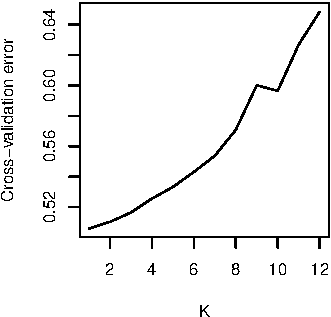
\includegraphics{plot/unnamed-chunk-13-1.pdf}
\caption{Cross-validation error as a function of K for the example
dataset.}
\end{figure}

The cross-validation error suggests a single source population can model
the data adequately and larger values of \(K\) lead to over-fitting.

To inspect further, we can use the \texttt{pong} software to visualize
the ancestry components inferred at different \(K\) across sevderal
runs. We need to set-up some the results and input files first.

\begin{Shaded}
\begin{Highlighting}[]
\CommentTok{# Run for different values of K, each with 10 runs}
\VariableTok{prefix=}\NormalTok{H938_Euro.LDprune}
\KeywordTok{for} \ExtensionTok{r}\NormalTok{ in }\DataTypeTok{\{1..10\}}\KeywordTok{;} \KeywordTok{do} \KeywordTok{for} \ExtensionTok{K}\NormalTok{ in }\DataTypeTok{\{2..12\}}\KeywordTok{;} 
\KeywordTok{do} 
  \ExtensionTok{admixture}\NormalTok{ -s }\VariableTok{$\{RANDOM\}}\NormalTok{ out/}\VariableTok{$\{prefix\}}\NormalTok{.bed }\VariableTok{$K}
  \FunctionTok{mv}\NormalTok{ out/}\VariableTok{$\{prefix\}}\NormalTok{.}\VariableTok{$\{K\}}\NormalTok{.Q out/}\VariableTok{$\{prefix\}}\NormalTok{.K}\VariableTok{$\{K\}}\NormalTok{r}\VariableTok{$\{r\}}\NormalTok{.Q}
\KeywordTok{done}\NormalTok{; }\KeywordTok{done} 

\CommentTok{# create Qmap file for pong}
\FunctionTok{createQmap()}\KeywordTok{\{}
\BuiltInTok{local} \VariableTok{r=$1}
\BuiltInTok{local} \VariableTok{K=$2}
\FunctionTok{awk}\NormalTok{ -v K=}\VariableTok{$K}\NormalTok{ -v r=}\VariableTok{$r}\NormalTok{ -v file=}\VariableTok{$\{prefix\}}\NormalTok{.K}\VariableTok{$\{K\}}\NormalTok{r}\VariableTok{$\{r\}} \StringTok{'BEGIN\{ \textbackslash{}}
\StringTok{printf("K%dr%d\textbackslash{}t%d\textbackslash{}t%s.Q\textbackslash{}n",K,r,K,file)}
\StringTok{\}'} \OperatorTok{>>}\NormalTok{ out/}\VariableTok{$\{prefix\}}\NormalTok{.multiplerun.Qfilemap}
\KeywordTok{\}}
\BuiltInTok{export}\NormalTok{ -f }\VariableTok{createQmap}
\KeywordTok{for} \ExtensionTok{K}\NormalTok{ in }\DataTypeTok{\{2..12\}}\KeywordTok{;} \KeywordTok{do} \KeywordTok{for} \ExtensionTok{r}\NormalTok{ in }\DataTypeTok{\{1..10\}}\KeywordTok{;} \KeywordTok{do} \ExtensionTok{createQmap} \VariableTok{$r} \VariableTok{$K}\KeywordTok{;} \KeywordTok{\textbackslash{}}
\KeywordTok{done}\NormalTok{; }\KeywordTok{done}

\CommentTok{#run pong}
\ExtensionTok{pong}\NormalTok{ -m out/H938_Euro.LDprune.multiplerun.Qfilemap --greedy \textbackslash{}}
\NormalTok{-s.95 -i out/H938_Euro.ind2pop}
\end{Highlighting}
\end{Shaded}

\begin{figure}
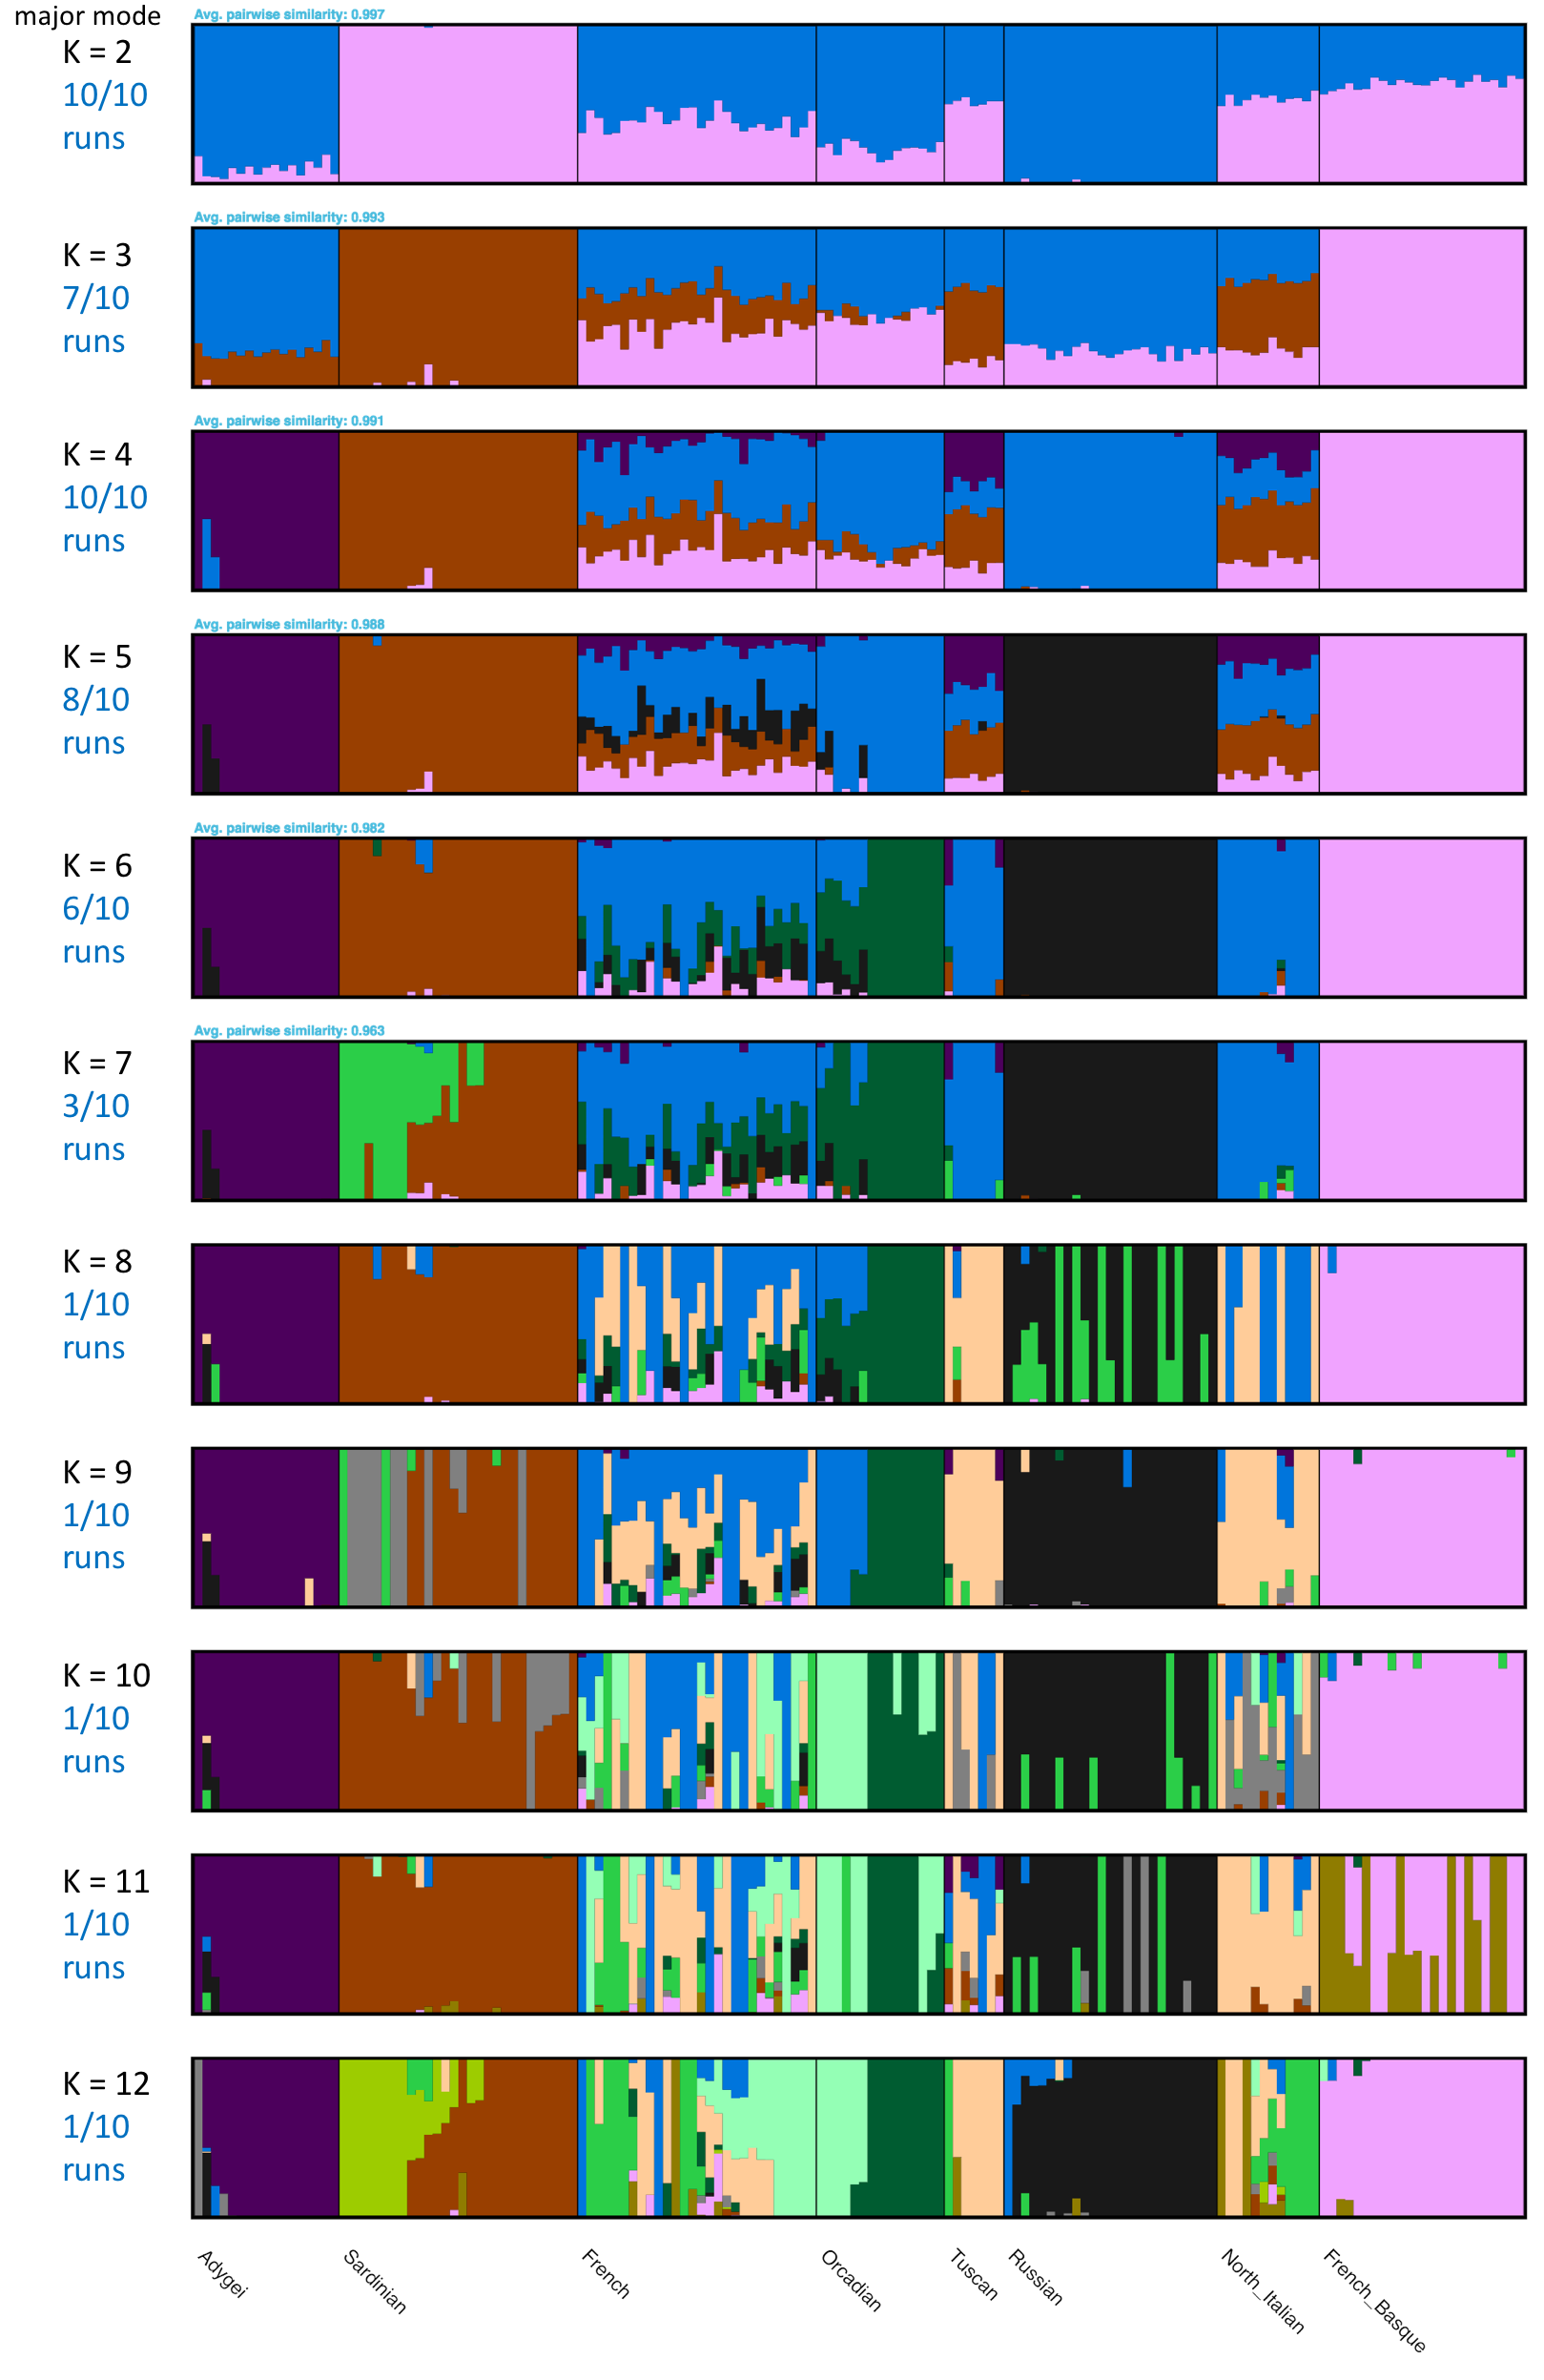
\includegraphics[width=1\linewidth]{./plot/H938_Euro_LDprune_12K_10r} \caption{Example PONG output showing results from across a range of K values (with ten ADMIXTURE runs per K value)}\label{fig:unnamed-chunk-15}
\end{figure}

Here we find how as \(K\) increases through to \(K=6\), the Sardinian,
Basque, Adygei, and Russian samples are typically modeled as descended
from unique sources, and at \(K\) of 7, 8, 9 we find structure within
the Sardinian, Russian, Orcadian, and Basque samples is revealed, though
for each, the substructure is not very stable. The values of \(K=10\)
and above make increasingly finer scale divisions that are difficult to
interpret, and the major modesfor \(K=7\) and up only consist of one to
three runs, suggesting a very multi-modal likelihood surface and a poor
resolution of the population structure.

Overall, its interesting to note that the visual inspection of the
results suggests several ``real'' clusters in the data, supported by an
alignment of the clustering with known population labels, even though
the cross-validation supports a value of \(K=1\). This highlights a
long-standing known issue with admixutre modeling: the selection of
\(K\) is a difficult problem to automate in a way that is robust.

\subsubsection{Some advanced options}\label{some-advanced-options}

Running \texttt{ADMIXTURE} with the \texttt{-B} option provides
estimates of standard errors on the ancestry proportion inferences. The
\texttt{-l} flag runs \texttt{ADMIXTURE} with a penalized likelihood
that favors more sparse solutions (i.e., ancestry proportions that are
closer to zero). This is useful in settings where small, possibly
erroneous ancestry proportions may be overinterpreted. By using the
\texttt{-P} option, the population allele frequencies inferred from one
dataset can be provided as input for inference of admixture proportions
in a second dataset. This is useful when individuals of unknown ancestry
are being analyzed against the background of a reference sample set.
Please see the \texttt{ADMIXTURE} manual for a complete listing of
options and more detail, and we encourage testing these options in test
datasets such as the one provided here.

\subsection{PCA with SMARTPCA}\label{pca-with-smartpca}

\subsubsection{Running PCA}\label{running-pca}

Comparing ADMIXTURE and PCA results often helps give insight and
confirmation regarding population structure in a sample. To run PCA, a
standard package that is well-suited for SNP data is the
\texttt{smartpca} package maintained by Nick Patterson and Alkes Price
(at \url{http://data.broadinstitute.org/alkesgroup/EIGENSOFT/}). To run
it, we first set-up a basic \texttt{smartpca} parameter file from the
command-line of a \texttt{bash} shell:

\begin{Shaded}
\begin{Highlighting}[]
\VariableTok{PREFIX=}\NormalTok{H938_Euro.LDprune}
\BuiltInTok{echo}\NormalTok{ genotypename: out/}\VariableTok{$PREFIX}\NormalTok{.bed }\OperatorTok{>}\NormalTok{ out/}\VariableTok{$PREFIX}\NormalTok{.par}
\BuiltInTok{echo}\NormalTok{ snpname: out/H938_Euro.LDprune.bim }\OperatorTok{>>}\NormalTok{ out/}\VariableTok{$PREFIX}\NormalTok{.par}
\BuiltInTok{echo}\NormalTok{ indivname: out/H938_Euro.LDprune.PCA.fam }\OperatorTok{>>}\NormalTok{ out/}\VariableTok{$PREFIX}\NormalTok{.par}
\BuiltInTok{echo}\NormalTok{ snpweightoutname: out/H938_Euro.LDprune.snpeigs \textbackslash{}}
\OperatorTok{>>}\NormalTok{ out/}\VariableTok{$PREFIX}\NormalTok{.par}
\BuiltInTok{echo}\NormalTok{ evecoutname: out/H938_Euro.LDprune.eigs }\OperatorTok{>>}\NormalTok{ out/}\VariableTok{$PREFIX}\NormalTok{.par}
\BuiltInTok{echo}\NormalTok{ evaloutname: out/H938_Euro.LDprune.eval }\OperatorTok{>>}\NormalTok{ out/}\VariableTok{$PREFIX}\NormalTok{.par}
\BuiltInTok{echo}\NormalTok{ phylipoutname: out/H938_Euro.LDprune.fst }\OperatorTok{>>}\NormalTok{ out/}\VariableTok{$PREFIX}\NormalTok{.par}
\BuiltInTok{echo}\NormalTok{ numoutevec: 20 }\OperatorTok{>>}\NormalTok{ out/}\VariableTok{$PREFIX}\NormalTok{.par}
\BuiltInTok{echo}\NormalTok{ numoutlieriter: 0 }\OperatorTok{>>}\NormalTok{ out/}\VariableTok{$PREFIX}\NormalTok{.par}
\BuiltInTok{echo}\NormalTok{ outlieroutname: out/H938_Euro.LDprune.out }\OperatorTok{>>}\NormalTok{ out/}\VariableTok{$PREFIX}\NormalTok{.par}
\BuiltInTok{echo}\NormalTok{ altnormstyle: NO }\OperatorTok{>>}\NormalTok{ out/}\VariableTok{$PREFIX}\NormalTok{.par}
\BuiltInTok{echo}\NormalTok{ missingmode: NO }\OperatorTok{>>}\NormalTok{ out/}\VariableTok{$PREFIX}\NormalTok{.par}
\BuiltInTok{echo}\NormalTok{ nsnpldregress: 0 }\OperatorTok{>>}\NormalTok{ out/}\VariableTok{$PREFIX}\NormalTok{.par}
\BuiltInTok{echo}\NormalTok{ noxdata: YES }\OperatorTok{>>}\NormalTok{ out/}\VariableTok{$PREFIX}\NormalTok{.par}
\BuiltInTok{echo}\NormalTok{ nomalexhet: YES }\OperatorTok{>>}\NormalTok{ out/}\VariableTok{$PREFIX}\NormalTok{.par}
\end{Highlighting}
\end{Shaded}

This input parameter file runs \texttt{smartpca} in its most basic mode
(i.e.~no automatic outlier removal or adjustments for LD - features
which you might want to explore later).

As a minor issue, \texttt{smartpca} ignores individuals in the
\texttt{.fam} file if they are marked as missing in the phenotypes
column. This \texttt{awk} command provides a new \texttt{.fam} file that
will automatically include all individuals.

\begin{Shaded}
\begin{Highlighting}[]
\FunctionTok{awk} \StringTok{'\{print $1,$2,$3,$4,$5,1\}'}\NormalTok{ out/H938_Euro.LDprune.fam \textbackslash{}}
\OperatorTok{>}\NormalTok{ out/H938_Euro.LDprune.PCA.fam}
\end{Highlighting}
\end{Shaded}

Now run \texttt{smartpca} with the following command.

\begin{Shaded}
\begin{Highlighting}[]
\ExtensionTok{smartpca}\NormalTok{ -p ./out/H938_Euro.LDprune.par}
\end{Highlighting}
\end{Shaded}

You will find the output files in the \texttt{out} sub-directory as
specified in the parameter file.

\subsubsection{Plotting PCA results with
PCAviz}\label{plotting-pca-results-with-pcaviz}

The PCAviz package can be found at
\url{https://github.com/NovembreLab/PCAviz}. It provides a simple
interface for quickly creating plots from PCA results. It encodes
several of our favored best practices for plotting PCA (such as using
abbreviations for point characters and plotting median positions of each
labelled group). To install the package use:

\begin{Shaded}
\begin{Highlighting}[]
\KeywordTok{install.packages}\NormalTok{(}\StringTok{"devtools"}\NormalTok{)}
\NormalTok{devtools}\OperatorTok{::}\KeywordTok{install_github}\NormalTok{(}\StringTok{"NovembreLab/PCAviz"}\NormalTok{,}
                         \DataTypeTok{build_vignettes =} \OtherTok{TRUE}\NormalTok{)}
\end{Highlighting}
\end{Shaded}

The following command in \texttt{R} generates plots showing each
individual sample's position in the PCA space and the median position of
each labelled group in PCA space:

\begin{Shaded}
\begin{Highlighting}[]
\KeywordTok{library}\NormalTok{(PCAviz)}
\KeywordTok{library}\NormalTok{(cowplot)}
\NormalTok{prefix <-}\StringTok{ "out/H938_Euro.LDprune"}
\NormalTok{nPCs <-}\StringTok{ }\DecValTok{20}

\CommentTok{# Read in individual coordinates on PCs and eignvalues}
\NormalTok{PCA <-}\StringTok{ }\KeywordTok{read.table}\NormalTok{(}\KeywordTok{paste}\NormalTok{(prefix, }\StringTok{".eigs"}\NormalTok{, }\DataTypeTok{sep =} \StringTok{""}\NormalTok{))}
\KeywordTok{names}\NormalTok{(PCA) <-}\StringTok{ }\KeywordTok{c}\NormalTok{(}\StringTok{"ID"}\NormalTok{, }\KeywordTok{paste}\NormalTok{(}\StringTok{"PC"}\NormalTok{, (}\DecValTok{1}\OperatorTok{:}\NormalTok{nPCs), }\DataTypeTok{sep =} \StringTok{""}\NormalTok{), }
                  \StringTok{"case.control"}\NormalTok{)}
\NormalTok{PCA <-}\StringTok{ }\NormalTok{PCA[, }\DecValTok{1}\OperatorTok{:}\NormalTok{(nPCs }\OperatorTok{+}\StringTok{ }\DecValTok{1}\NormalTok{)] }\CommentTok{# Remove case/control column}
\NormalTok{eig.val <-}\StringTok{ }\KeywordTok{sqrt}\NormalTok{(}\KeywordTok{unlist}\NormalTok{(}\KeywordTok{read.table}\NormalTok{(}
  \KeywordTok{paste}\NormalTok{(prefix, }\StringTok{".eval"}\NormalTok{, }\DataTypeTok{sep =} \StringTok{""}\NormalTok{)))[}\DecValTok{1}\OperatorTok{:}\NormalTok{nPCs])}
\NormalTok{sum.eig <-}\StringTok{ }\KeywordTok{sum}\NormalTok{(}\KeywordTok{unlist}\NormalTok{(}\KeywordTok{read.table}\NormalTok{(}
  \KeywordTok{paste}\NormalTok{(prefix, }\StringTok{".eval"}\NormalTok{, }\DataTypeTok{sep =} \StringTok{""}\NormalTok{))))}

\CommentTok{# Read in snp weightings matrix}
\NormalTok{snpeigs <-}\StringTok{ }\KeywordTok{read.table}\NormalTok{(}\KeywordTok{paste}\NormalTok{(prefix, }\StringTok{".snpeigs"}\NormalTok{, }\DataTypeTok{sep =} \StringTok{""}\NormalTok{))}
\KeywordTok{names}\NormalTok{(snpeigs) <-}\StringTok{ }\KeywordTok{c}\NormalTok{(}\StringTok{"ID"}\NormalTok{, }\StringTok{"chr"}\NormalTok{, }\StringTok{"pos"}\NormalTok{, }
                    \KeywordTok{paste}\NormalTok{(}\StringTok{"PC"}\NormalTok{, (}\DecValTok{1}\OperatorTok{:}\NormalTok{nPCs), }\DataTypeTok{sep =} \StringTok{""}\NormalTok{))}
\NormalTok{snpeigs}\OperatorTok{$}\NormalTok{chr <-}\StringTok{ }\KeywordTok{factor}\NormalTok{(snpeigs}\OperatorTok{$}\NormalTok{chr)}
\KeywordTok{rownames}\NormalTok{(snpeigs) <-}\StringTok{ }\NormalTok{snpeigs}\OperatorTok{$}\NormalTok{ID}
\NormalTok{snpeigs <-}\StringTok{ }\NormalTok{snpeigs[, }\DecValTok{-1}\NormalTok{]}

\CommentTok{# Note smartpca pushes the plink family and individual}
\CommentTok{# ids together so we need to extract out the ids afresh}
\NormalTok{tmp <-}\StringTok{ }\KeywordTok{unlist}\NormalTok{(}\KeywordTok{sapply}\NormalTok{(}\KeywordTok{as.character}\NormalTok{(PCA}\OperatorTok{$}\NormalTok{ID), strsplit, }\StringTok{":"}\NormalTok{))}
\NormalTok{ids <-}\StringTok{ }\NormalTok{tmp[}\KeywordTok{seq}\NormalTok{(}\DecValTok{2}\NormalTok{, }\KeywordTok{length}\NormalTok{(tmp), }\DataTypeTok{by =} \DecValTok{2}\NormalTok{)]}
\NormalTok{PCA}\OperatorTok{$}\NormalTok{ID <-}\StringTok{ }\NormalTok{ids}

\CommentTok{# Read in the group/cluster labels}
\NormalTok{clst <-}\StringTok{ }\KeywordTok{read.table}\NormalTok{(}\StringTok{"out/Euro.clst.txt"}\NormalTok{)}
\CommentTok{# Order them to match the ids of PCA object}
\NormalTok{clst_unord <-}\StringTok{ }\NormalTok{clst}\OperatorTok{$}\NormalTok{V3[}\KeywordTok{match}\NormalTok{(ids, clst}\OperatorTok{$}\NormalTok{V2)] }
\NormalTok{PCA <-}\StringTok{ }\KeywordTok{as.data.frame}\NormalTok{(PCA)}
\NormalTok{PCA <-}\StringTok{ }\KeywordTok{cbind}\NormalTok{(PCA, clst_unord)}
\KeywordTok{names}\NormalTok{(PCA)[}\KeywordTok{ncol}\NormalTok{(PCA)] <-}\StringTok{ "sample"}

\CommentTok{# Build the PCAviz object}
\NormalTok{hgdp <-}\StringTok{ }\KeywordTok{pcaviz}\NormalTok{(}\DataTypeTok{dat =}\NormalTok{ PCA, }\DataTypeTok{sdev =}\NormalTok{ eig.val, }
               \DataTypeTok{var =}\NormalTok{ sum.eig, }\DataTypeTok{rotation =}\NormalTok{ snpeigs)}
\NormalTok{hgdp <-}\StringTok{ }\KeywordTok{pcaviz_abbreviate_var}\NormalTok{(hgdp, }\StringTok{"sample"}\NormalTok{)}

\CommentTok{# Make PCA plots}
\NormalTok{geom.point.summary.params <-}\StringTok{ }\KeywordTok{list}\NormalTok{(}
  \DataTypeTok{shape =} \DecValTok{16}\NormalTok{, }\DataTypeTok{stroke =} \DecValTok{1}\NormalTok{, }\DataTypeTok{size =} \DecValTok{5}\NormalTok{,}
  \DataTypeTok{alpha =} \FloatTok{.7}\NormalTok{, }\DataTypeTok{show.legend =}\NormalTok{ F}
\NormalTok{)}
\NormalTok{plot1 <-}\StringTok{ }\KeywordTok{plot}\NormalTok{(hgdp,}
  \DataTypeTok{coords =} \KeywordTok{paste0}\NormalTok{(}\StringTok{"PC"}\NormalTok{, }\KeywordTok{c}\NormalTok{(}\DecValTok{1}\NormalTok{, }\DecValTok{2}\NormalTok{)), }\DataTypeTok{color =} \StringTok{"sample"}\NormalTok{,}
  \DataTypeTok{geom.point.summary.params =}\NormalTok{ geom.point.summary.params, }
  \DataTypeTok{scale.pc.axes =} \FloatTok{0.6}
\NormalTok{)}
\NormalTok{plot2 <-}\StringTok{ }\KeywordTok{plot}\NormalTok{(hgdp,}
  \DataTypeTok{coords =} \KeywordTok{paste0}\NormalTok{(}\StringTok{"PC"}\NormalTok{, }\KeywordTok{c}\NormalTok{(}\DecValTok{2}\NormalTok{, }\DecValTok{3}\NormalTok{)), }\DataTypeTok{color =} \StringTok{"sample"}\NormalTok{,}
  \DataTypeTok{geom.point.summary.params =}\NormalTok{ geom.point.summary.params, }
  \DataTypeTok{scale.pc.axes =} \FloatTok{0.6}
\NormalTok{)}
\NormalTok{plot3 <-}\StringTok{ }\KeywordTok{plot}\NormalTok{(hgdp,}
  \DataTypeTok{coords =} \KeywordTok{paste0}\NormalTok{(}\StringTok{"PC"}\NormalTok{, }\KeywordTok{c}\NormalTok{(}\DecValTok{4}\NormalTok{, }\DecValTok{5}\NormalTok{)), }\DataTypeTok{color =} \StringTok{"sample"}\NormalTok{,}
  \DataTypeTok{geom.point.summary.params =}\NormalTok{ geom.point.summary.params, }
  \DataTypeTok{scale.pc.axes =} \FloatTok{0.6}
\NormalTok{)}
\NormalTok{plot4 <-}\StringTok{ }\KeywordTok{plot}\NormalTok{(hgdp,}
  \DataTypeTok{coords =} \KeywordTok{paste0}\NormalTok{(}\StringTok{"PC"}\NormalTok{, }\KeywordTok{c}\NormalTok{(}\DecValTok{5}\NormalTok{, }\DecValTok{6}\NormalTok{)), }\DataTypeTok{color =} \StringTok{"sample"}\NormalTok{,}
  \DataTypeTok{geom.point.summary.params =}\NormalTok{ geom.point.summary.params, }
  \DataTypeTok{scale.pc.axes =} \FloatTok{0.6}
\NormalTok{)}

\KeywordTok{plot_grid}\NormalTok{(plot1, plot2, plot3, plot4)}
\end{Highlighting}
\end{Shaded}

\begin{figure}
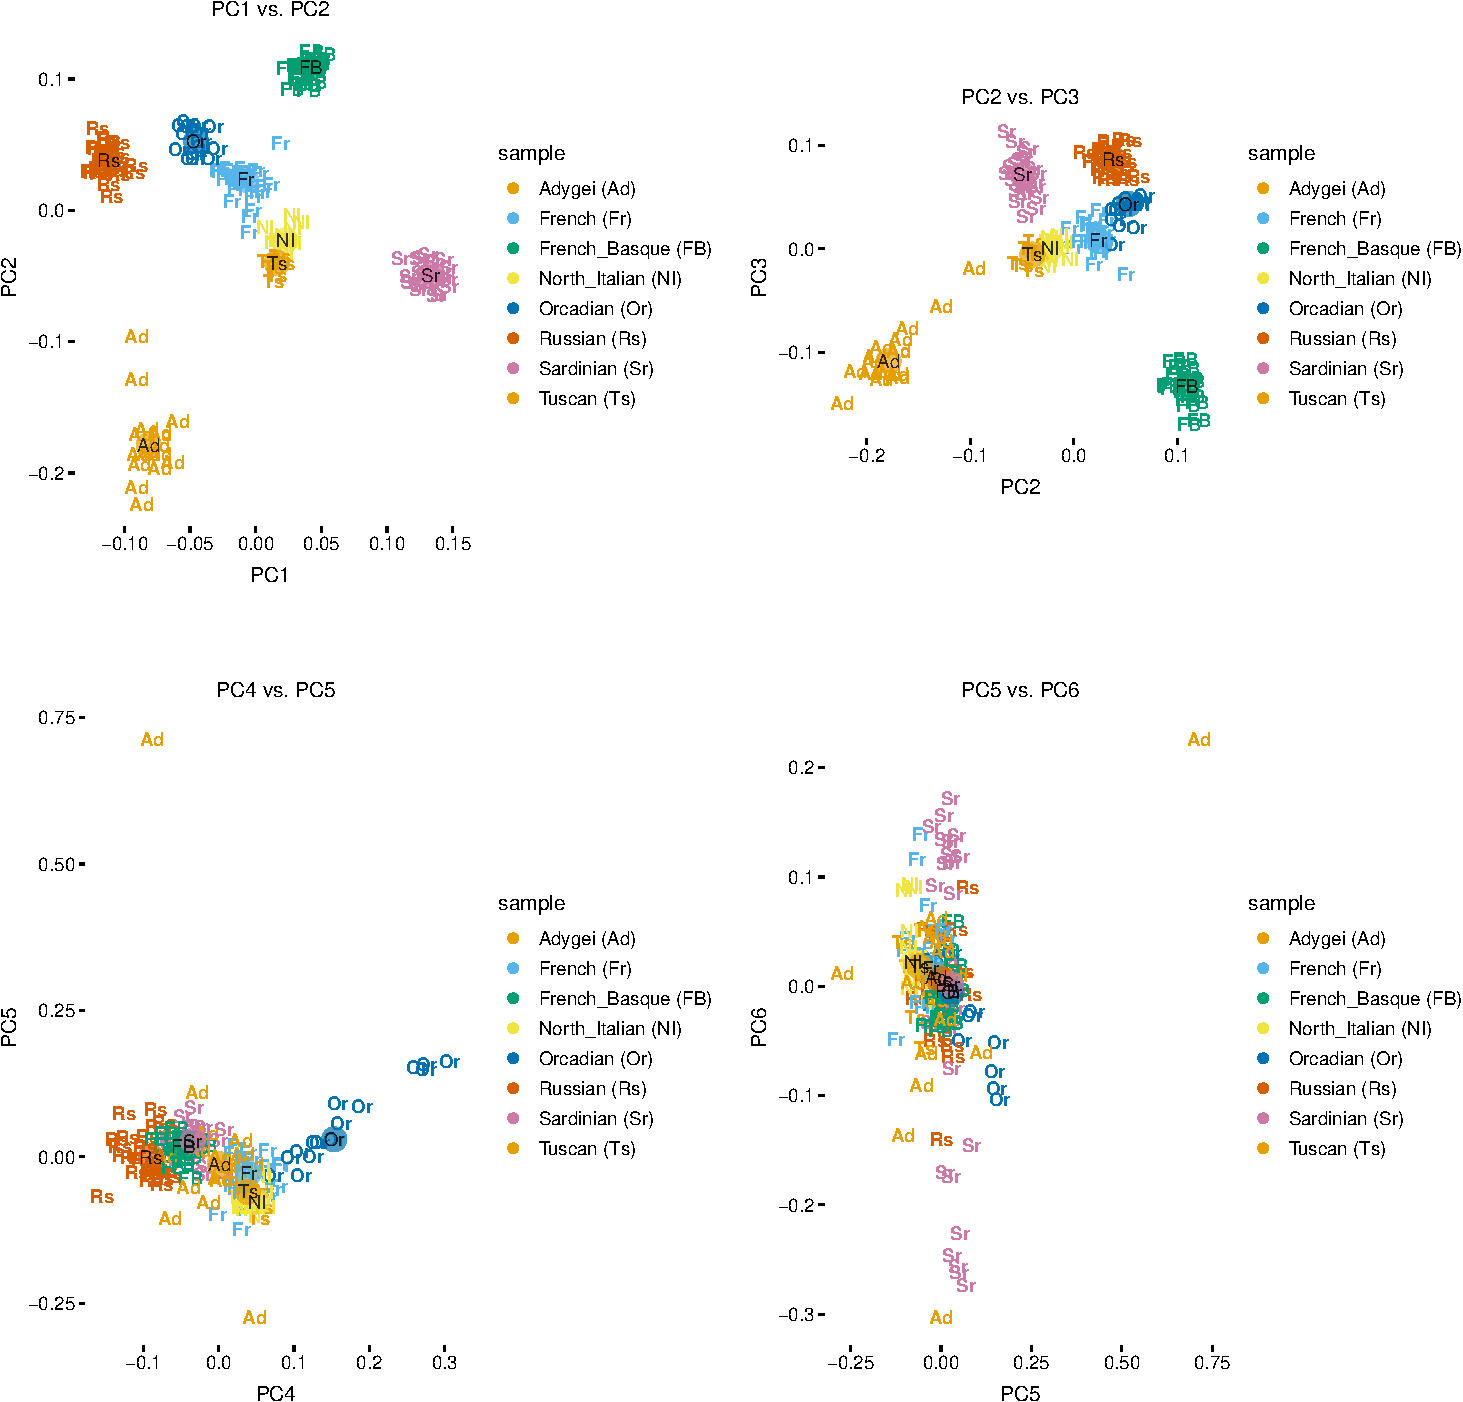
\includegraphics[width=1\linewidth]{plot/unnamed-chunk-20-1} \caption{Pairwise plots of PC scores generated using the PCAviz package.}\label{fig:unnamed-chunk-20}
\end{figure}

First one may notice several populations are separated with PC1 and PC2,
with the more isolated populations being those that were most
distinguished from the others by \texttt{ADMIXTURE}. PC4 distinguishes a
subset of Orcadian individuals and PC5 distinguishes two Adygei
individuals. PC6 corresponds to the cryptic structure observed within
Sardinians in the \texttt{ADMIXTURE} analysis.

As an alternative visualization, it can be helpful to see the
distribution of PC coordinates per population for each labelled group in
the data:

\begin{Shaded}
\begin{Highlighting}[]
\KeywordTok{pcaviz_violin}\NormalTok{(hgdp, }\DataTypeTok{pc.dims =} \KeywordTok{paste0}\NormalTok{(}\StringTok{"PC"}\NormalTok{, }\KeywordTok{c}\NormalTok{(}\DecValTok{1}\OperatorTok{:}\DecValTok{3}\NormalTok{)), }
              \DataTypeTok{plot.grid.params =} \KeywordTok{list}\NormalTok{(}\DataTypeTok{nrow =} \DecValTok{3}\NormalTok{))}
\end{Highlighting}
\end{Shaded}

\begin{figure}
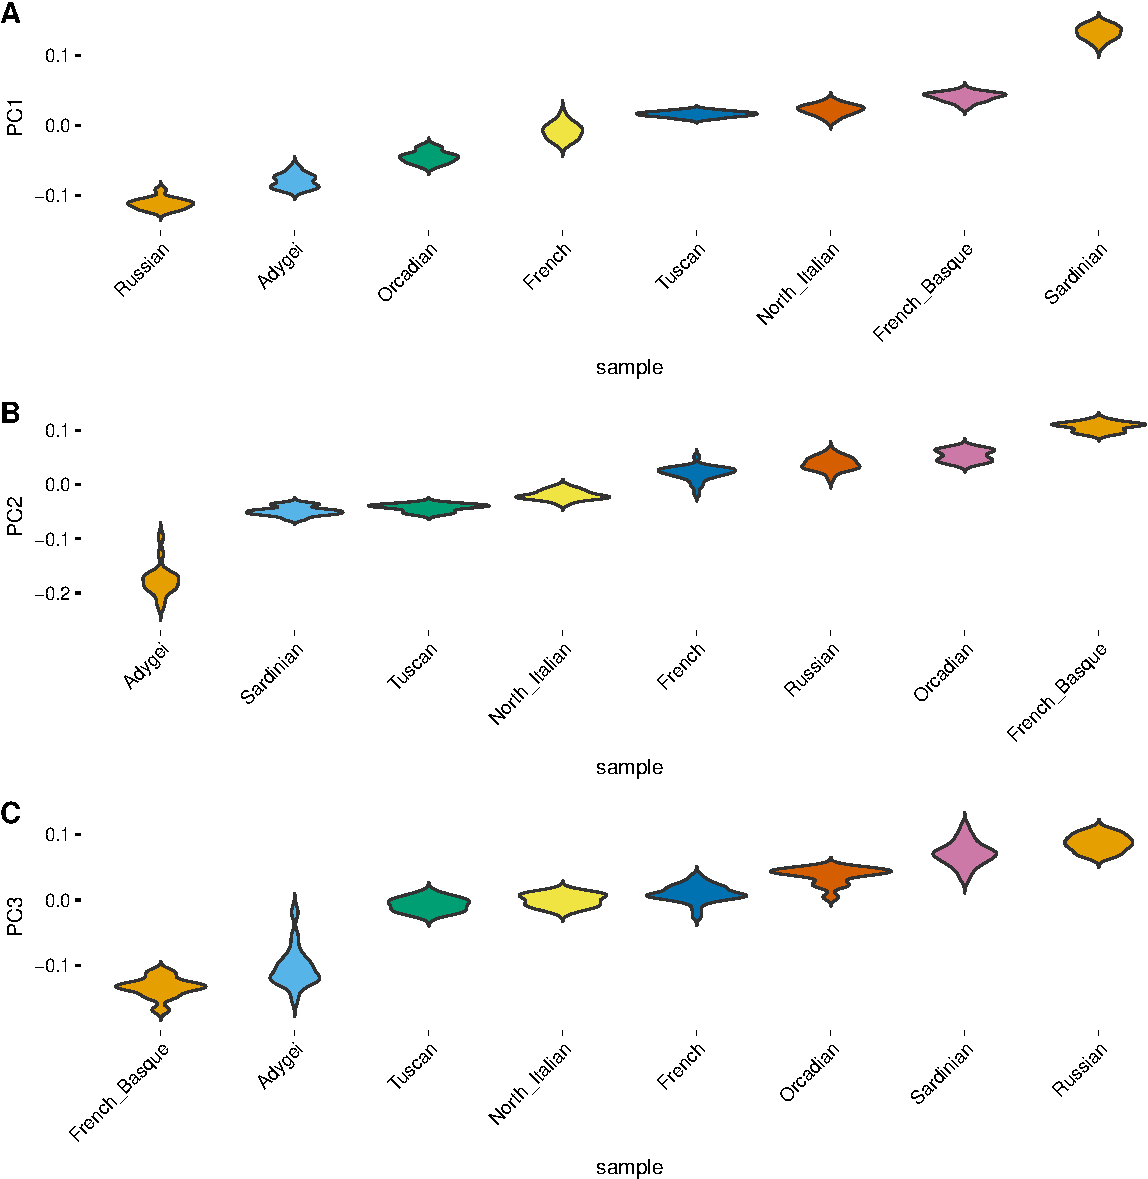
\includegraphics[width=1\linewidth]{plot/unnamed-chunk-21-1} \caption{Violin plots of PC values generated using the PCAviz package.}\label{fig:unnamed-chunk-21}
\end{figure}

As mentioned above in the section on LD, it is useful to inspect the PC
loadings to ensure that they broadly represent variation across the
genome, rather than one or a small number of genomic regions
(Duforet-Frebourg et al. 2016). SNPs that are selected in the same
direction as genome-wide structure can show high loadings, but what is
particularly pathological is if the only SNPs that show high loadings
are all concentrated in a single region of the genome, as might occur if
the PCA is explaining genomic structure (such as an inversion) rather
than population structure.

\begin{Shaded}
\begin{Highlighting}[]
\ControlFlowTok{for}\NormalTok{ (i }\ControlFlowTok{in} \DecValTok{1}\OperatorTok{:}\DecValTok{5}\NormalTok{) \{}
\NormalTok{  plotname <-}\StringTok{ }\KeywordTok{paste}\NormalTok{(}\StringTok{"plot"}\NormalTok{, i, }\DataTypeTok{sep =} \StringTok{""}\NormalTok{)}
\NormalTok{  plot <-}\StringTok{ }\KeywordTok{pcaviz_loadingsplot}\NormalTok{(hgdp,}
    \DataTypeTok{pc.dim =} \KeywordTok{paste0}\NormalTok{(}\StringTok{"PC"}\NormalTok{, i),}
    \DataTypeTok{min.rank =} \FloatTok{0.8}\NormalTok{, }\DataTypeTok{gap =} \DecValTok{200}\NormalTok{, }\DataTypeTok{color =} \StringTok{"chr"}\NormalTok{,}
    \DataTypeTok{geom.point.params =} \KeywordTok{list}\NormalTok{(}\DataTypeTok{show.legend =} \OtherTok{FALSE}\NormalTok{)}
\NormalTok{  ) }\OperatorTok{+}
\StringTok{    }\KeywordTok{xlab}\NormalTok{(}\StringTok{"SNPs"}\NormalTok{) }\OperatorTok{+}\StringTok{ }\KeywordTok{ylab}\NormalTok{(}\KeywordTok{paste0}\NormalTok{(}\StringTok{"PC"}\NormalTok{, i, }\StringTok{" loading"}\NormalTok{))}
  \KeywordTok{assign}\NormalTok{(plotname, plot)}
\NormalTok{\}}
\CommentTok{# grep common legend}
\NormalTok{plot <-}\StringTok{ }\KeywordTok{pcaviz_loadingsplot}\NormalTok{(hgdp,}
  \DataTypeTok{pc.dim =} \KeywordTok{paste0}\NormalTok{(}\StringTok{"PC"}\NormalTok{, }\DecValTok{1}\NormalTok{),}
  \DataTypeTok{min.rank =} \FloatTok{0.8}\NormalTok{, }\DataTypeTok{gap =} \DecValTok{200}\NormalTok{, }\DataTypeTok{color =} \StringTok{"chr"}
\NormalTok{) }\OperatorTok{+}
\StringTok{  }\KeywordTok{guides}\NormalTok{(}\DataTypeTok{color =} \KeywordTok{guide_legend}\NormalTok{(}\DataTypeTok{nrow =} \DecValTok{2}\NormalTok{, }\DataTypeTok{byrow =} \OtherTok{TRUE}\NormalTok{)) }\OperatorTok{+}
\StringTok{  }\KeywordTok{theme}\NormalTok{(}\DataTypeTok{legend.position =} \StringTok{"bottom"}\NormalTok{, }
        \DataTypeTok{legend.justification =} \StringTok{"center"}\NormalTok{)}
\NormalTok{plot_legend <-}\StringTok{ }\KeywordTok{get_legend}\NormalTok{(plot)}
\CommentTok{# plot loadings}
\NormalTok{prow <-}\StringTok{ }\KeywordTok{plot_grid}\NormalTok{(plot1, plot2, plot3, plot4, plot5,}
                  \DataTypeTok{nrow =} \DecValTok{5}\NormalTok{, }\DataTypeTok{align =} \StringTok{"vh"}\NormalTok{)}
\KeywordTok{plot_grid}\NormalTok{(prow, plot_legend, }\DataTypeTok{ncol =} \DecValTok{1}\NormalTok{, }\DataTypeTok{rel_heights =} \KeywordTok{c}\NormalTok{(}\DecValTok{1}\NormalTok{, }\FloatTok{.2}\NormalTok{))}
\end{Highlighting}
\end{Shaded}

\begin{figure}
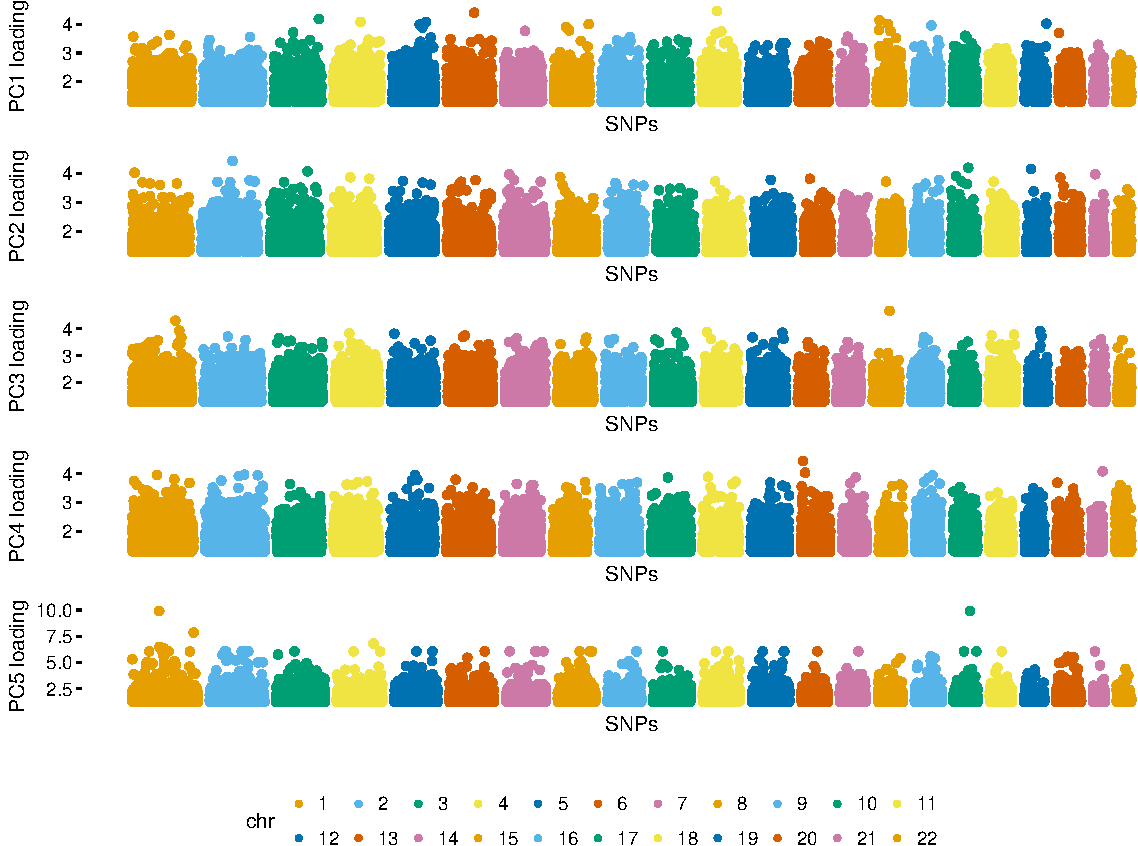
\includegraphics[width=1\linewidth]{plot/unnamed-chunk-22-1} \caption{PC loading plots generated using the PCAviz package.}\label{fig:unnamed-chunk-22}
\end{figure}

The proportion of total variance explained by each PC is a useful metric
for understanding structure in a sample and for evaluating how many PCs
one might want to include in downstream analyses. This can be computed
as \(\lambda_i / \sum_{k} \lambda_k\), with \(\lambda_i\) being
eigenvalues in decreasing order, and is plotted below:

\begin{Shaded}
\begin{Highlighting}[]
\KeywordTok{screeplot}\NormalTok{(hgdp, }\DataTypeTok{type =} \StringTok{"pve"}\NormalTok{) }\OperatorTok{+}\StringTok{ }
\StringTok{  }\KeywordTok{ylim}\NormalTok{(}\DecValTok{0}\NormalTok{, }\FloatTok{0.018}\NormalTok{) }\OperatorTok{+}
\StringTok{  }\KeywordTok{ylab}\NormalTok{(}\StringTok{'Proportion of Variance Explained'}\NormalTok{) }\OperatorTok{+}
\StringTok{  }\KeywordTok{theme}\NormalTok{(}\DataTypeTok{axis.text.x =} \KeywordTok{element_text}\NormalTok{(}\DataTypeTok{angle =} \DecValTok{90}\NormalTok{, }\DataTypeTok{hjust =} \DecValTok{1}\NormalTok{)) }\OperatorTok{+}
\StringTok{  }\KeywordTok{theme}\NormalTok{(}\DataTypeTok{axis.line =} \KeywordTok{element_line}\NormalTok{(}\DataTypeTok{size =} \DecValTok{1}\NormalTok{, }\DataTypeTok{linetype =} \StringTok{"solid"}\NormalTok{))}
\end{Highlighting}
\end{Shaded}

\begin{verbatim}
## Scale for 'y' is already present. Adding another scale for 'y', which
## will replace the existing scale.
\end{verbatim}

\begin{figure}
\centering
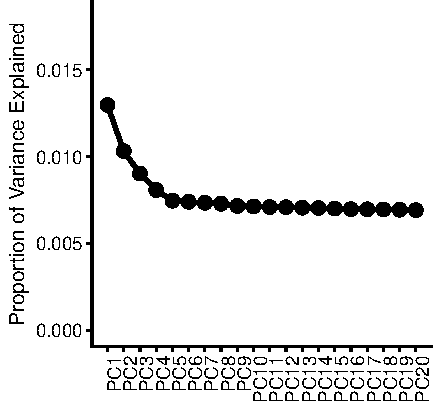
\includegraphics{plot/unnamed-chunk-23-1.pdf}
\caption{Proportion of variance explained by each PC. Plot generated
using the PCAviz package.}
\end{figure}

The results show that the top PCs only explain a small fraction of the
variance (\textless{}1.5\%) and that after about \(K=6\) the variance
explained per PC becomes relatively constant; roughly in line with the
visual inspection of the \texttt{admixture} results that revealed
\(K=6\) may be reasonable for this dataset.

\section{Discussion}\label{discussion}

Our protocol above is relatively straightforward and presents the most
basic implementation of these analyses. Each analysis sofware
(\texttt{ADMIXTURE} and \texttt{smartpca}) and each visualization
package (\texttt{pong} and \texttt{PCAviz}) contain numerous other
options that may be suitable for specific analyses and we encourage the
readers to spend time in the manuals of each. Nonetheless, what we have
presented is a useful start and a standard pipeline that we use in our
research.

Two broad perspectives we find helpful useful to keep in mind are: 1)
How the admixture model and PCA framework are related to each other
indirectly as different forms of sparse factor analysis (Engelhardt and
Stephens 2010); 2) How the PCA framework in particular can be considered
as a form of efficient data compression. Both of these perspectives can
be helpful in interpreting the outputs of the methods and for
appreciating how these approaches best serve as helpful visual
exploratory tools for analyzing structure in genetic data. These methods
are ultimately relatively simple statistical tools being used to
summarize complex realities. They are part of the toolkit for analysis,
and often are extremely useful for framing specific models of population
structure that can be further investigated using more detailed and
explicit approaches (such as those based on coalescent or diffusion
theory, Chapters 7 on MSMC and 8 on CoalHMM).

\bibliographystyle{spmpsci}
\bibliography{references}

\end{document}
